%需使用xelatex编译
%导言区
\documentclass[UTF8,hyperref,space=auto]{ctexart} %UTF8编码,引入hyperref宏包(可形成超链接及使用其自带的额外命令),设置其处理空格的方式为auto
\usepackage[a4paper,showframe]{geometry} %设置纸张为A4大小
\usepackage[dvipsnames]{xcolor} %扩展版的颜色宏包
\usepackage{cprotect} %保护被抄录的语句
\usepackage{lipsum} %形成一些随机的英语文字
\usepackage{zhlipsum} %形成一些随机的中文文字
\usepackage{amsmath} %数学命令及环境中最重要的宏包之一
\usepackage{amssymb} %输出更多的数学符号
\usepackage{mathtools} %提供了dcases环境
\usepackage{extarrows} %提供了更多的数学长箭头
\usepackage{multirow} %提供可跨行的处理表格的命令
\usepackage{array} %提供了更多的表格列说明符,以及修正了一些表格显示上的问题
\usepackage{booktabs} %以使用学术上常见的三线表命令
\usepackage{graphicx} %插图专用宏包
\graphicspath{{figures/}} %图片在当前目录的figures目录下
\usepackage{caption,subcaption} %输出子图表专用
\usepackage{float} %其H参数可以让浮动环境不再浮动
\usepackage{titlesec,titletoc} %可分别设置目录和正文中的标题样式
\usepackage{natbib} %专门用来排版文献的宏包
\usepackage[nottoc]{tocbibind} %默认可将参考文献、索引等放入tableofcontents
\usepackage[amsmath,thmmarks]{ntheorem} %定理类环境宏包,如果前面使用amsmath宏包,则需加上amsmath宏包选项以避免出现未知问题,若需在定理环境末尾加上特定符号(如证毕符号),则需使用thmmarks宏包选项以使用\theoremsymbol{}命令。


%定理类环境设置(依赖于ntheorem宏包)
{
	\theoremstyle{plain}
	\setlength{\theoremindent}{2em}
	\newtheorem{definition}{定义}
}

{
	\theoremstyle{plain}
	\setlength{\theoremindent}{2em}
	\newtheorem{lemma}[definition]{引理}
}

{
	\theoremstyle{plain}
	\setlength{\theoremindent}{2em}
	\newtheorem{theorem}[definition]{定理}
}

{
	\theoremstyle{plain}
	\setlength{\theoremindent}{2em}
	\newtheorem{corollary}[definition]{推论}
}

{
	\theoremstyle{nonumberplain}
	\setlength{\theoremindent}{2em}
	\theorembodyfont{\normalfont}
	\theoremsymbol{$\blacksquare$} %在证明环境末尾加上一个证毕符号
	\newtheorem{proof}{证明}
}


%标题页设置
\title{
	这个是文章的标题(This is a title)\\
	\large ——这个是文章的副标题(This is a subtitle)
}

\author{王美庭\thanks{王美庭,暨南大学经济与社会研究院,电子信箱:wangmeiting92@gmail.com}} %在独立的提名页中,用致谢命令生成的脚注不附带一条脚注线
\date{\today}

%超链接设置(依赖于hyperref宏包)
\hypersetup{
	pdftitle={这是展示在 PDF 信息中的标题},
	pdfauthor={王美庭},
	colorlinks=true,
	pdfsubject={这是 PDF 的主题,类似于摘要。},
	pdfkeywords={关键词1, 关键词2, ...},
	urlcolor={[RGB]{25, 128, 230}},%设置网页超链接的颜色
	linkcolor={[RGB]{25, 128, 230}},%设置目录、脚注、ref等超链接的颜色
	citecolor={[RGB]{25, 128, 230}},%设置cite超链接的颜色
}

%ctex 设置
\CTEXsetup[name={附录},number={\Alph{section}}]{appendix}

%指定参考文献的排版样式
\bibliographystyle{gbt7714-author-year}

%定义新命令或数学运算符
\DeclareMathOperator{\diff}{d\!} %定义微分运算符
\renewcommand{\bibname}{参考文献} %将bibname设定为“参考文献”



%正文区
\begin{document}
\maketitle

\tableofcontents

\section{引言}
这个是引言部分,然后这里有一点脚注\footnote{这里是对文章对应部分的脚注。}。

\section{超链接}
百度:\url{https://www.baidu.com}。

这是\href{https://www.baidu.com}{百度}的链接。

\section{定理类环境}
这里介绍了常用了定理类环境,而这些环境需要先在导言区声明后才能在正文区使用。

\begin{definition}
	这是一个定义环境。This is a dfn env.
\end{definition}

\begin{lemma}
	这是一个引理环境。This is a lemma env.
\end{lemma}

\begin{theorem}
	这是一个定理环境。This is a thm env.
\end{theorem}

\begin{corollary}
	这是一个推论环境。This is a coro env.
\end{corollary}

\begin{proof}
	这是一个证明环境。This is a proof env.
\end{proof}


\section{列表类环境}
无序的 itemize 环境:
\begin{itemize}
	\item 中文
	\begin{itemize}
		\item 中文 1
		\item 中文 2
	\end{itemize}
	\item English
	\begin{itemize}
		\item Eng 1
		\item Eng 2
		\begin{itemize}
			\item Eng 2.1
			\item Eng 2.2
		\end{itemize}
	\end{itemize}
	\item français
\end{itemize}

有序的 enumerate 环境:
\begin{enumerate}
	\item 中文
	\begin{enumerate}
		\item 中文 1
		\item 中文 2
	\end{enumerate}
	\item English
	\begin{enumerate}
		\item Eng 1
		\item Eng 2
		\begin{enumerate}
			\item Eng 2.1
			\item Eng 2.2
		\end{enumerate}
	\end{enumerate}
	\item français
\end{enumerate}

使用关键字的 description 环境:
\begin{description}
	\item[中文] 中国的语言文字
	\item[English] The language of English
	\item[xxx] This is a xxx's description
\end{description}


\section{数学命令及环境}
行内公式如 $a+b=b+a$,行间公式如:
\[ A = \iiint\limits_{0<x,y,z<1} f(x,y,z) \diff x \diff y \diff z \]

单个公式且编号(equation 环境\footnote{eqution* 环境不会编号,其他的环境类似。}):
\begin{equation}
	\sum_{i=1}^{n} x_i = x_1 + x_2 + \cdots + x_n
\end{equation}

多行公式且编号(gather 环境\cprotect\footnote{可以在某一行公式的后面加上 \verb|\notag| 以阻止其编号。}):
\begin{gather}
	a+b = b+a \\
	x\times y = y\times x
\end{gather}

多行公式编号且在等号处对齐(align 环境):
\begin{align}
	x &= t + \cos t + 1 \\
	y &= 2\sin t
\end{align}

多行数学公式环境中排版多列在等号处对齐的公式(align 环境):
\begin{align}
	y &= t & x &= \cos t & x &= t \\
	y &= 2t & y &= \sin(t+1) & y &= \sin t
\end{align}

拆分单个公式(split 环境):
\begin{equation}
	\begin{split}
		\cos 2x &= \cos^2 x - \sin^2 x \\
		&= 2\cos^2 x - 1
	\end{split}
\end{equation}

分段函数:
\begin{equation}
	f(x) =
	\begin{cases}
		x + \frac{1}{2}, & x < 0 \\
		x^2 + 6, & x \ge 0
	\end{cases}
\end{equation}

mathtools 宏包则进一步提供了 dcases 环境,它保证每行公式都是显示格式的大小(\verb|\displaystyle|):
\begin{equation}
	f(x) =
	\begin{dcases}
		x + \frac{1}{2}, & x < 0 \\
		x^2 + 6, & x \ge 0
	\end{dcases}
\end{equation}


\section{表格类环境}

普通表格(tabular 环境):\\
\begin{tabular}{|c|*{5}{c|}}
	\hline
	数字 & 1 & 2 & 3 & 4 & 5 \\
	\hline
	字母 & A & B & C & D & E \\
	\hline
	天干 & 甲 & 乙 & 丙 & 丁 & 戊 \\
	\hline
\end{tabular}

带有跨行或跨列的表格(tabular 环境):\\
\begin{tabular}{|c|c|c|}
	\hline
	\multirow{2}*{姓名} & \multicolumn{2}{c|}{成绩} \\ \cline{2-3}
	& 语文 & 数学 \\ \hline
	张三 & 87 & 100 \\ \hline
	李四 & 95 & 83 \\ \hline
\end{tabular}

使用 center 环境将表格居中显示(tabular 环境):
\begin{center}
	\begin{tabular}{cccccc}
		\hline
		&\multicolumn{1}{c}{count}&\multicolumn{1}{c}{mean}&\multicolumn{1}{c}{sd}&\multicolumn{1}{c}{min}&\multicolumn{1}{c}{max}\\
		\hline
		price       &          74&    6165.257&    2949.496&        3291&       15906\\
		mpg         &          74&     21.2973&    5.785503&          12&          41\\
		weight      &          74&    3019.459&    777.1936&        1760&        4840\\
		rep78       &          69&    3.405797&    .9899323&           1&           5\\
		\hline
	\end{tabular}
\end{center}

设置表格宽度为版心宽度(tabular* 环境):
\begin{center}
	\begin{tabular*}{\linewidth}{@{\hskip\tabcolsep\extracolsep\fill}l*{1}{*{5}{>{$}c<{$}}}}
		\hline
		&\multicolumn{1}{c}{count}&\multicolumn{1}{c}{mean}&\multicolumn{1}{c}{sd}&\multicolumn{1}{c}{min}&\multicolumn{1}{c}{max}\\
		\hline
		price       &          74&    6165.257&    2949.496&        3291&       15906\\
		mpg         &          74&     21.2973&    5.785503&          12&          41\\
		weight      &          74&    3019.459&    777.1936&        1760&        4840\\
		rep78       &          69&    3.405797&    .9899323&           1&           5\\
		\hline
	\end{tabular*}
\end{center}

使用 table 环境创建浮动体并设置表格标题:
\begin{table}[H]
	\centering
	\caption{主要变量的描述性统计 1}
	\begin{tabular}{l*{5}{>{$}c<{$}}}
		\hline
		&\text{count}&\text{mean}&\text{sd}&\text{min}&\text{max}\\
		\hline
		price       &          74&    6165.257&    2949.496&        3291&       15906\\
		mpg         &          74&     21.2973&    5.785503&          12&          41\\
		weight      &          74&    3019.459&    777.1936&        1760&        4840\\
		rep78       &          69&    3.405797&    .9899323&           1&           5\\
		\hline
	\end{tabular}
\end{table}

使用 booktabs 宏包的三线表命令,以更符合学术规范,如表 \ref{tab:stat} 所示:
\begin{table}[H]
	\centering
	\caption{主要变量的描述性统计 2}\label{tab:stat}
	\begin{tabular}{l*{5}{>{$}c<{$}}}
		\toprule
		&\text{count}&\text{mean}&\text{sd}&\text{min}&\text{max}\\
		\midrule
		price       &          74&    6165.257&    2949.496&        3291&       15906\\
		mpg         &          74&     21.2973&    5.785503&          12&          41\\
		weight      &          74&    3019.459&    777.1936&        1760&        4840\\
		rep78       &          69&    3.405797&    .9899323&           1&           5\\
		\bottomrule
	\end{tabular}
\end{table}

表格并排,如表 \ref{tab:score} 和表 \ref{tiangan} 所示:
\begin{table}[H]
	\begin{minipage}[t]{0.5\textwidth}
		\centering
		\caption{这是一个表格}\label{tab:score}
		\begin{tabular}{|c|c|c|}
			\hline
			\multirow{2}*{姓名} & \multicolumn{2}{c|}{成绩} \\ \cline{2-3}
			& 语文 & 数学 \\ \hline
			张三 & 87 & 100 \\ \hline
			李四 & 95 & 83 \\ \hline
		\end{tabular}
	\end{minipage}
	\begin{minipage}[t]{0.5\textwidth}
		\centering
		\caption{这是另外一个表格}\label{tiangan}
		\begin{tabular}{|c|*{5}{c|}}
			\hline
			数字 & 1 & 2 & 3 & 4 & 5 \\
			\hline
			字母 & A & B & C & D & E \\
			\hline
			天干 & 甲 & 乙 & 丙 & 丁 & 戊 \\
			\hline
		\end{tabular}
	\end{minipage}
\end{table}

子表格并排,如表 \ref{tab:subtab} 所示:
\begin{table}[H]
	\caption{子表格环境}\label{tab:subtab}
	\begin{subtable}[t]{0.5\textwidth}
		\centering
		\caption{子表格 1}
		\begin{tabular}{|c|c|c|}
			\hline
			\multirow{2}*{姓名} & \multicolumn{2}{c|}{成绩} \\ \cline{2-3}
			& 语文 & 数学 \\ \hline
			张三 & 87 & 100 \\ \hline
			李四 & 95 & 83 \\ \hline
		\end{tabular}
	\end{subtable}
	\begin{subtable}[t]{0.5\textwidth}
		\centering
		\caption{子表格 2}
		\begin{tabular}{|c|*{5}{c|}}
			\hline
			数字 & 1 & 2 & 3 & 4 & 5 \\
			\hline
			字母 & A & B & C & D & E \\
			\hline
			天干 & 甲 & 乙 & 丙 & 丁 & 戊 \\
			\hline
		\end{tabular}
	\end{subtable}
\end{table}

\section{插图类命令}
将图片以不同的宽度插入\footnote{除了 width,我们可以设置 height 或 scale。}:\\
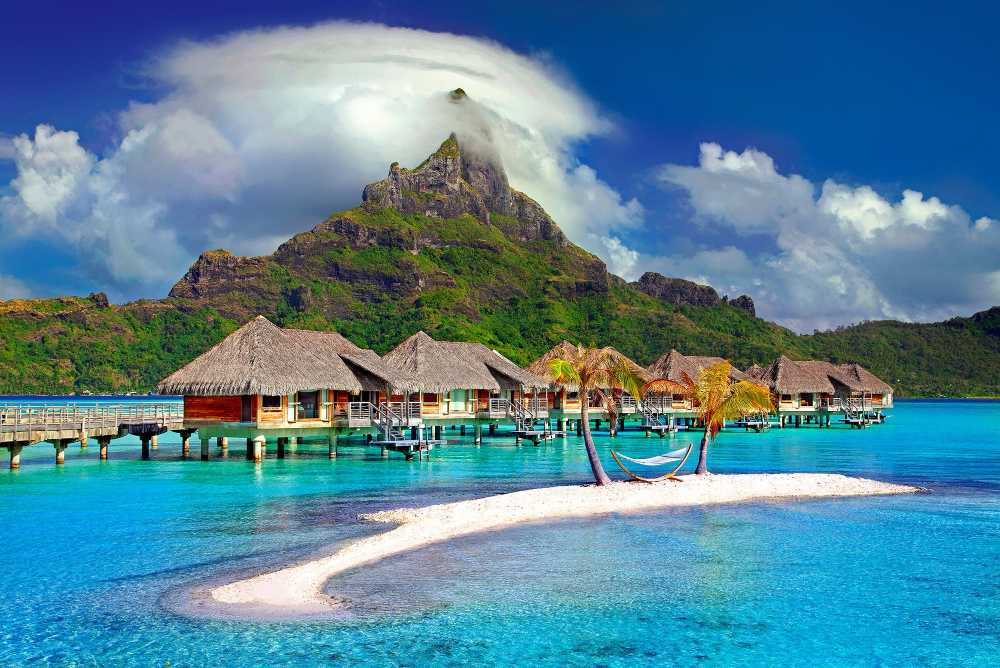
\includegraphics[width=2em]{1.jpg}
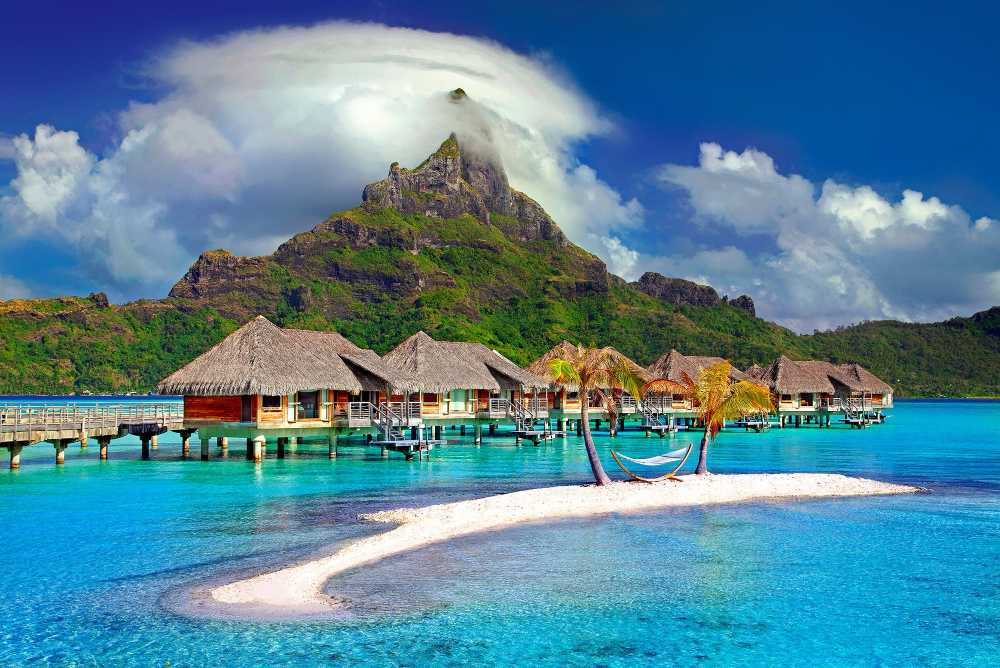
\includegraphics[width=4em]{1.jpg}
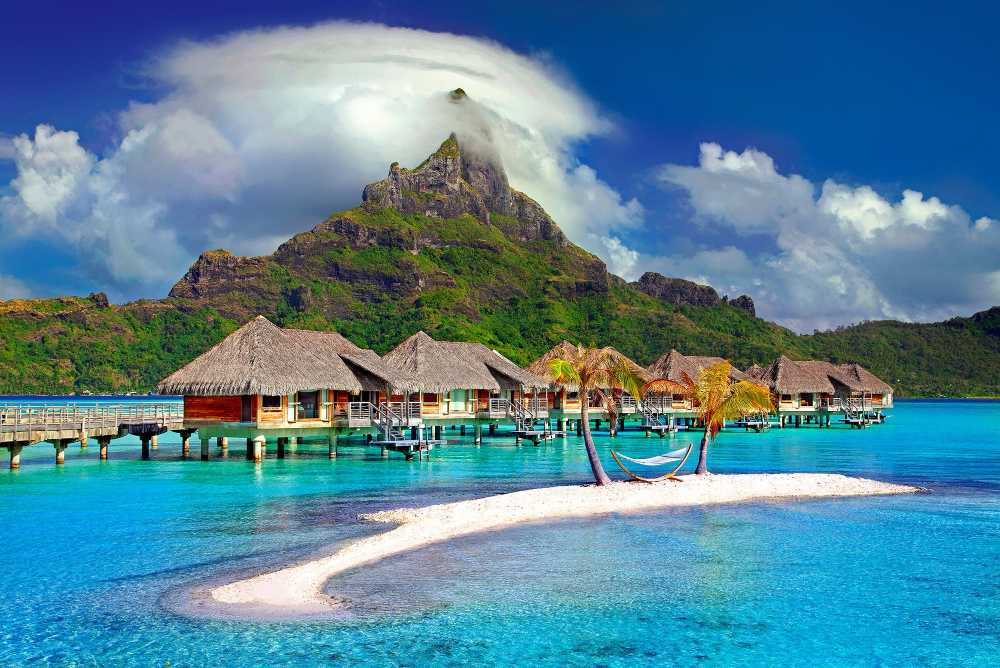
\includegraphics[width=6em]{1.jpg}
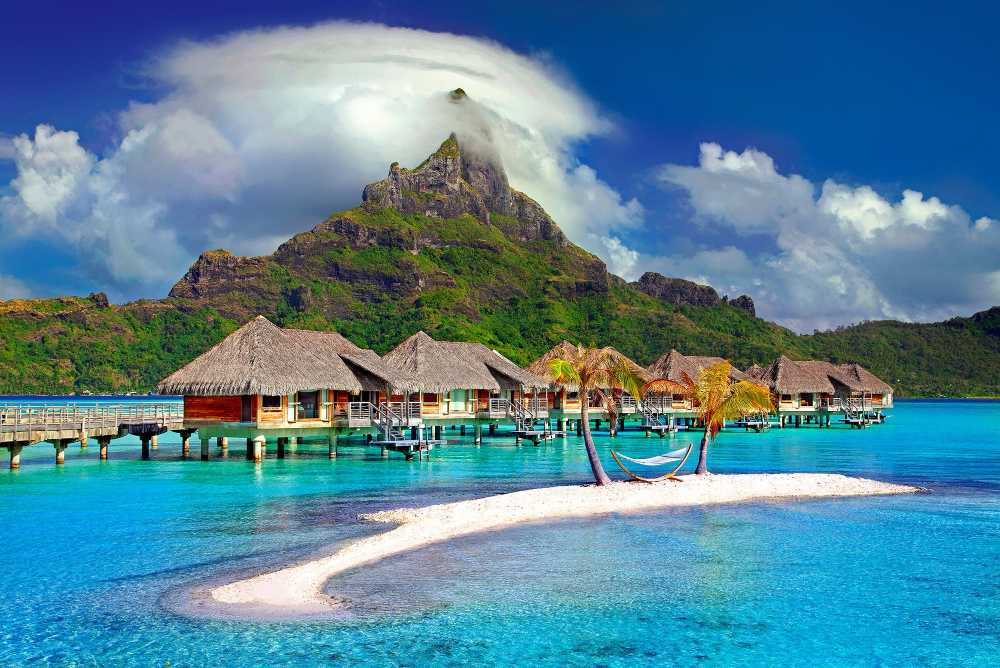
\includegraphics[width=8em]{1.jpg}
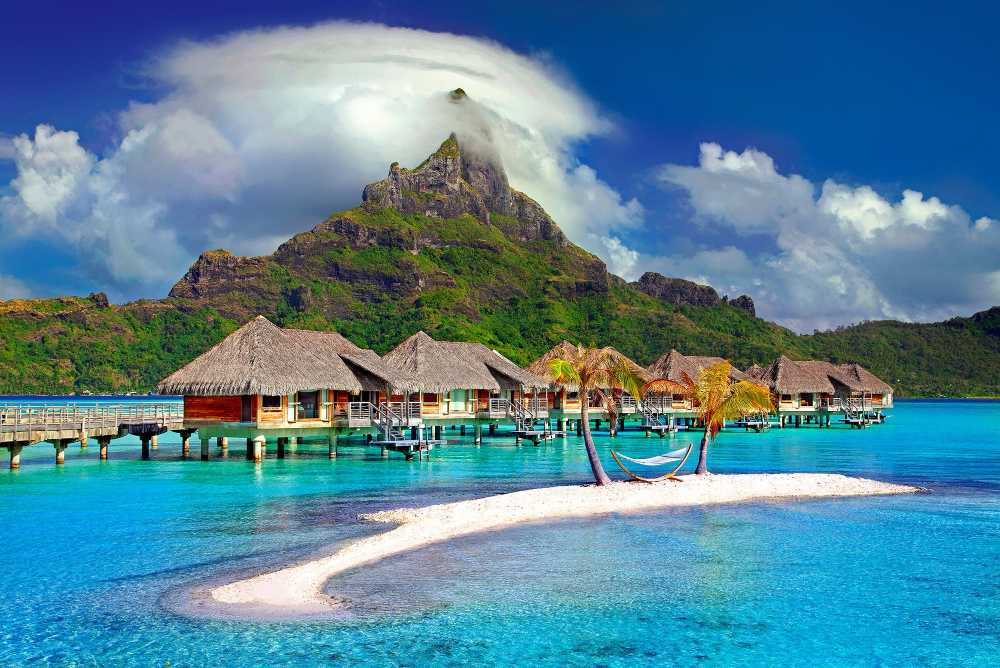
\includegraphics[width=10em]{1.jpg}

将图片放入浮动体中,并设定其宽度为 0.5 倍的版心宽度:
\begin{figure}[H]
	\centering
	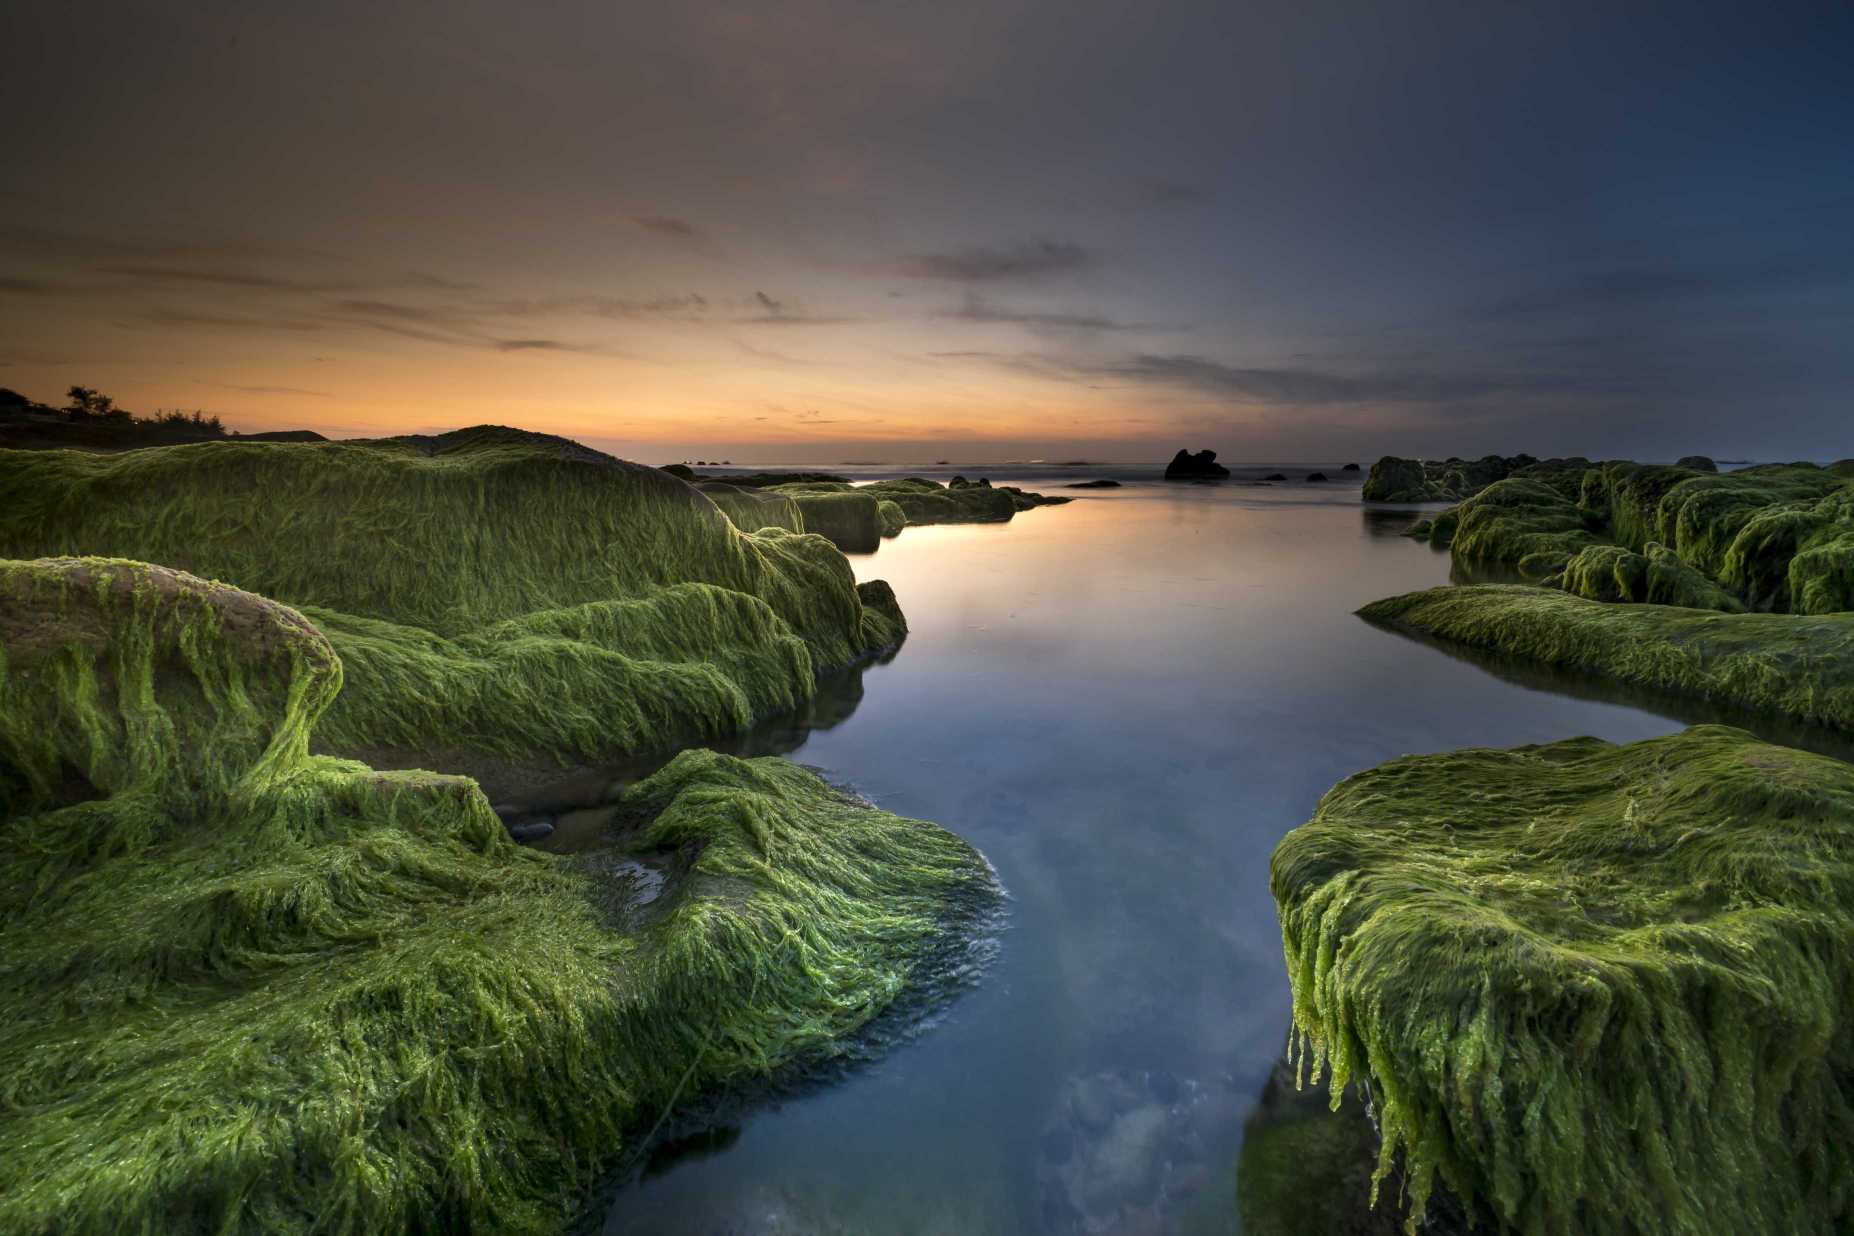
\includegraphics[width=0.5\linewidth]{2.jpg}
	\caption{This is a figure}
\end{figure}

图片并排:
\begin{figure}[H]
	\centering
	\begin{minipage}[t]{0.4\textwidth}
		\centering
		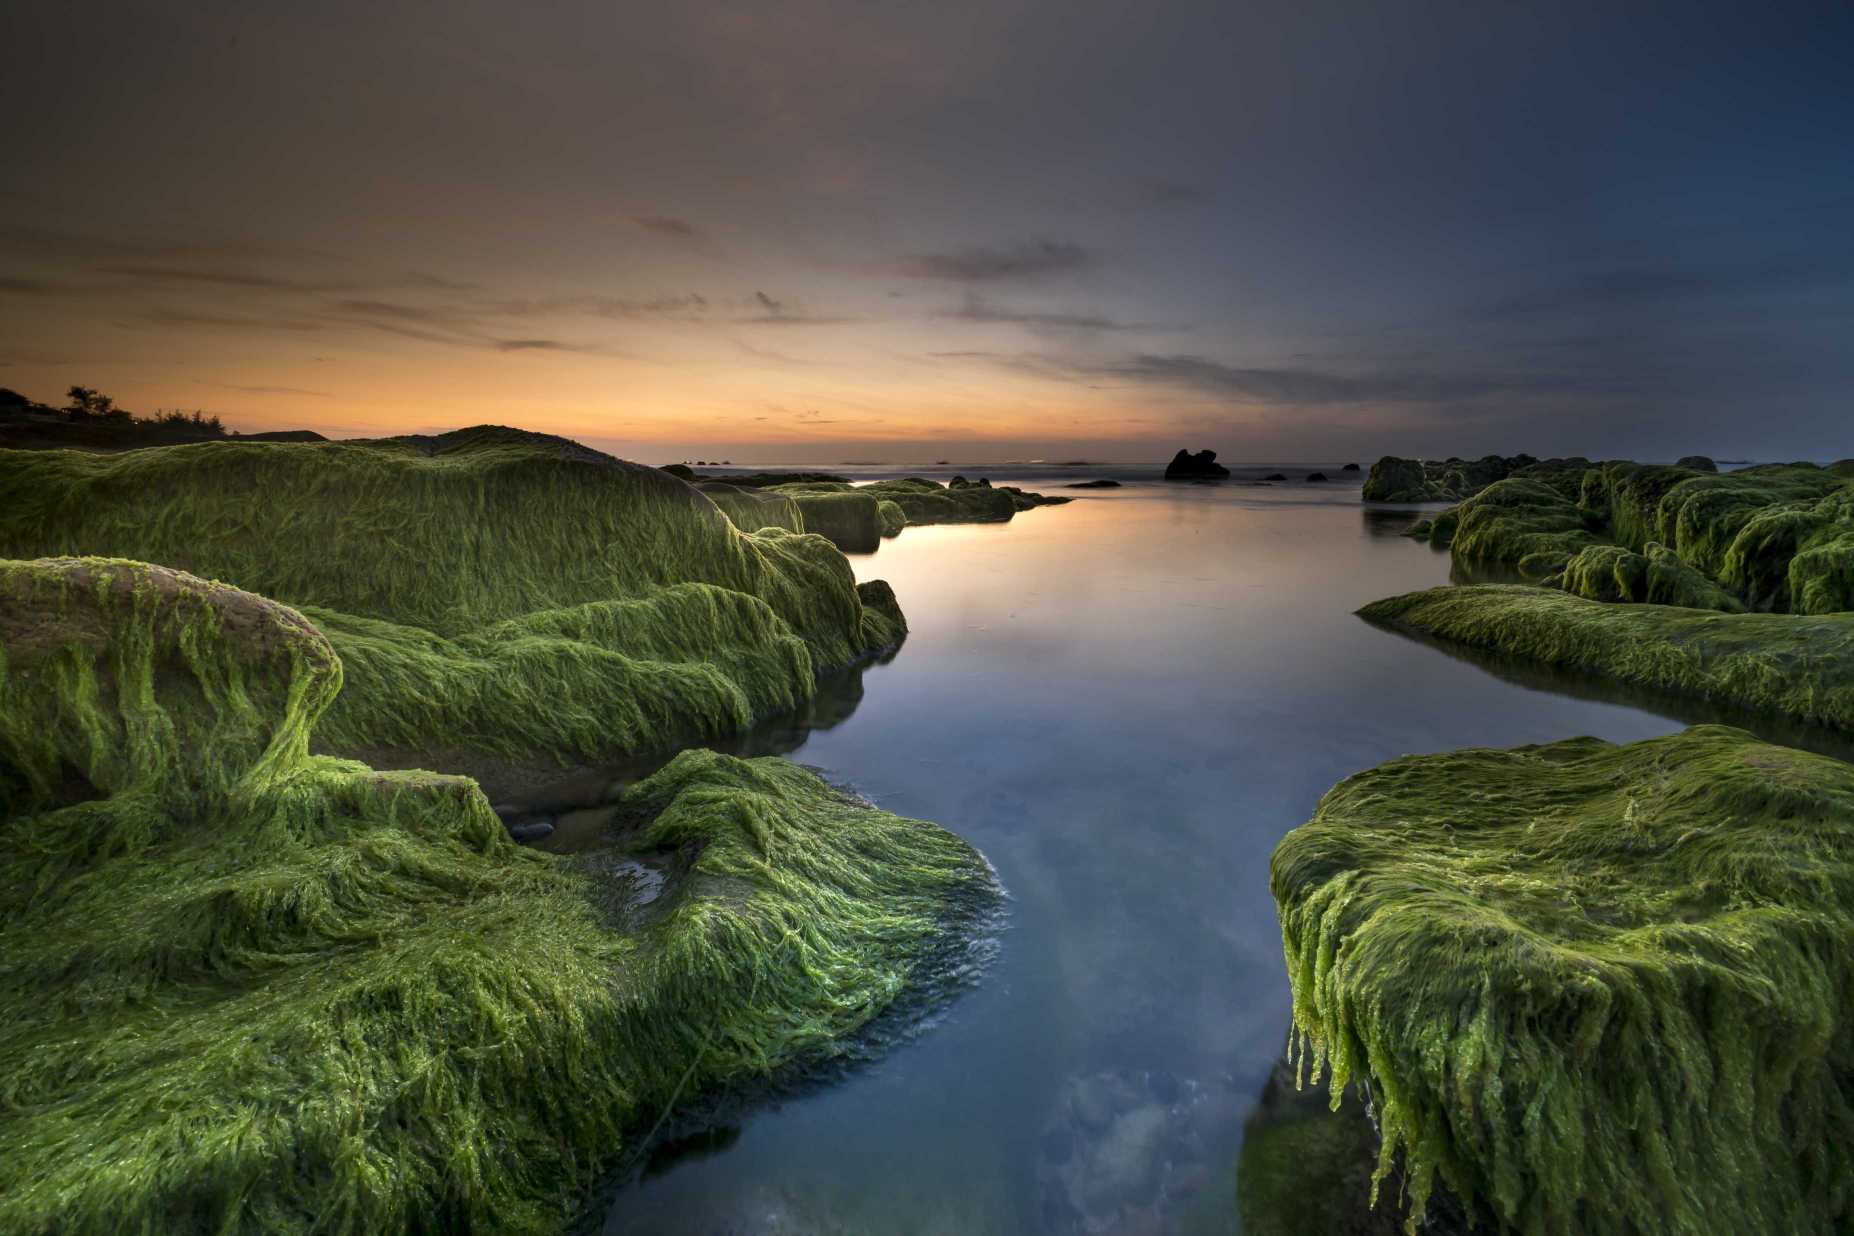
\includegraphics[width=\textwidth]{2.jpg}
		\caption{This is a figure}
	\end{minipage}
	\quad
	\begin{minipage}[t]{0.4\textwidth}
		\centering
		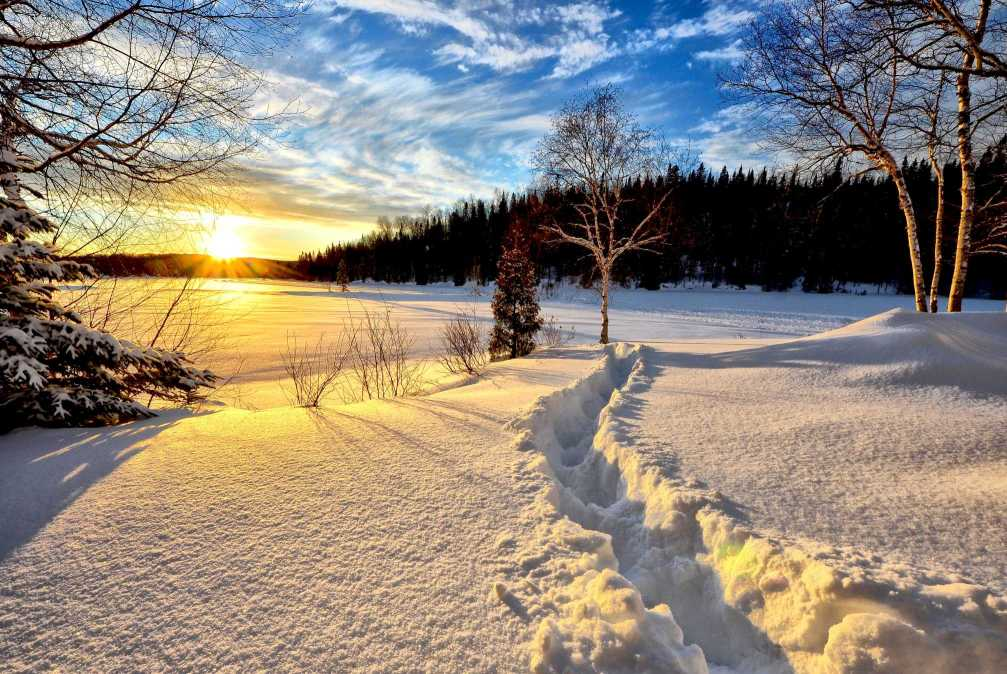
\includegraphics[width=\textwidth]{3.jpg}
		\caption{This is a figure too}
	\end{minipage}
\end{figure}

子图片并排:
\begin{figure}[H]
	\centering
	\begin{subtable}[t]{0.4\textwidth}
		\centering
		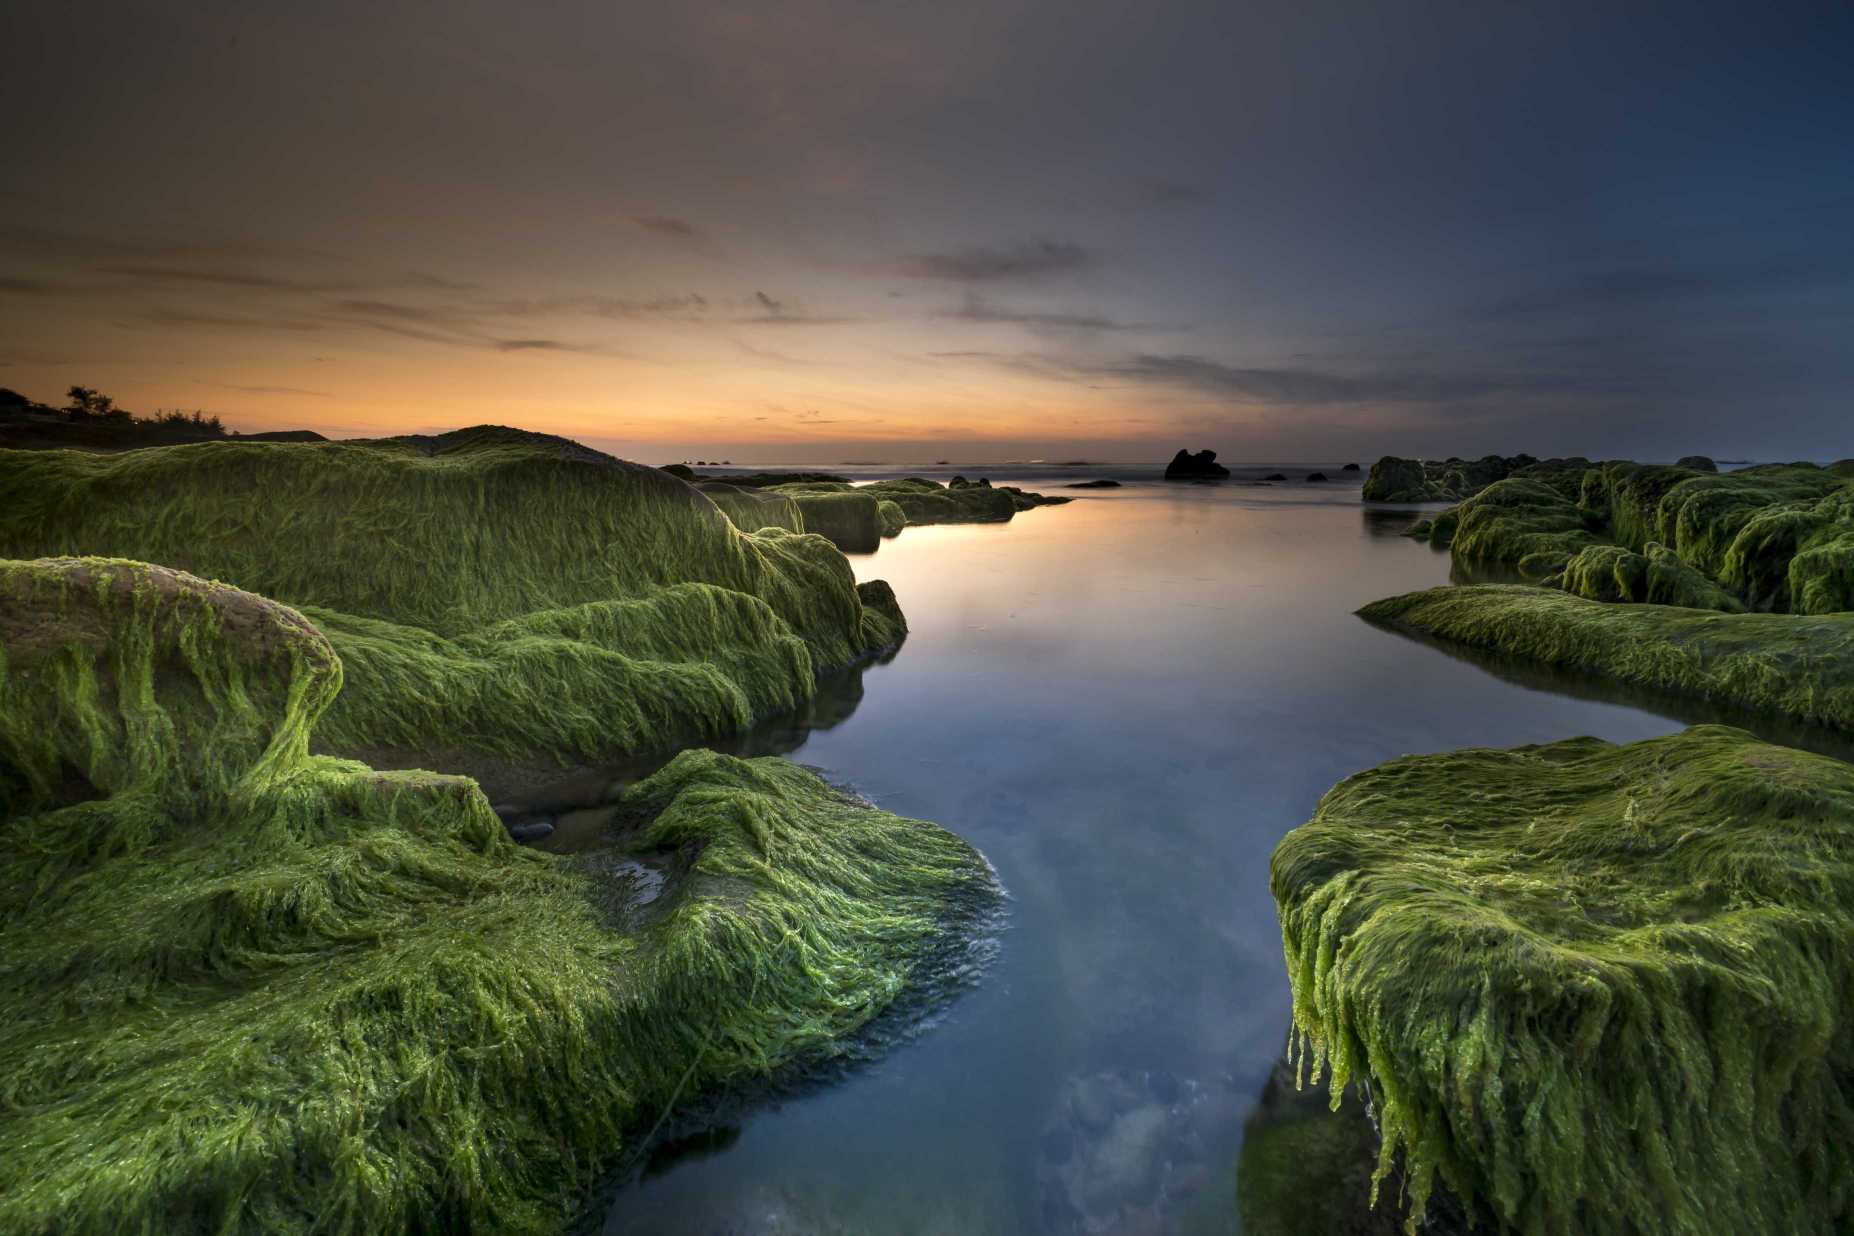
\includegraphics[width=\textwidth]{2.jpg}
		\caption{子图片 1}
	\end{subtable}
	\quad
	\begin{subtable}[t]{0.4\textwidth}
		\centering
		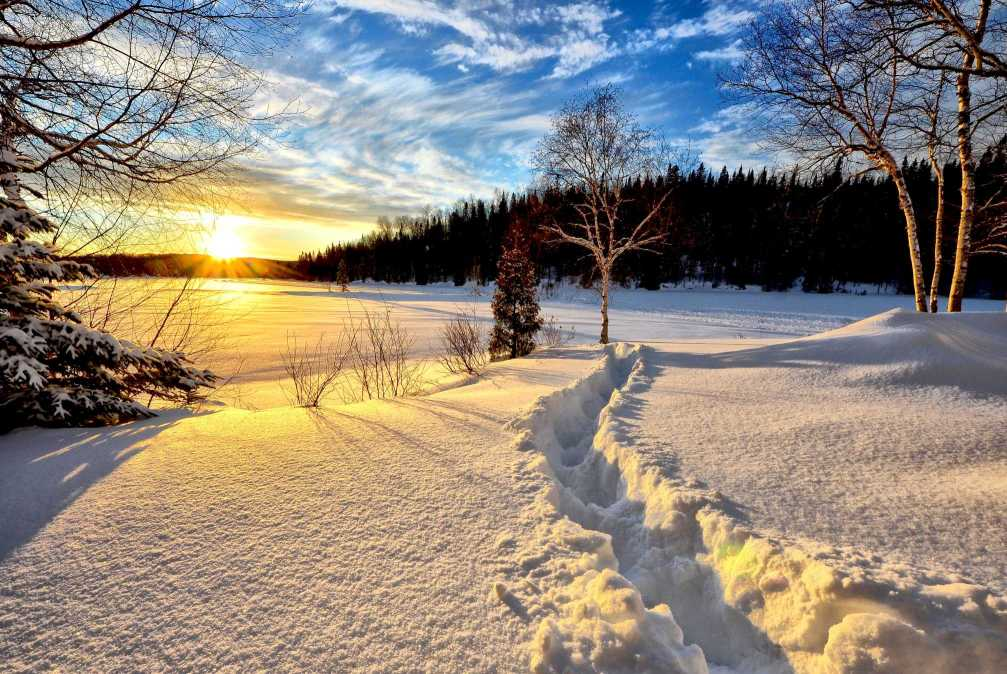
\includegraphics[width=\textwidth]{3.jpg}
		\caption{子图片 2}
	\end{subtable}
	\caption{子图片环境}
\end{figure}

\section{参考文献系列}
这是一篇文献的引用\citep{ChamonLiu-439},这又是另外一篇文献的引用\citep{李静潘丽群-420}。

\citet{JappelliPistaferri-433}指出,问题可以这样解决。

\citet{缪小林王婷-417}的研究表明,balalalala。

\citet{陆铭-455}的《大国大城》很有实际意义。


\bibliography{reference.bib} %在正文中需要输出参考文献的地方指定参考文献数据库
\nocite{*}


\appendix

\section{附录第一章}
这是附录第一章的内容。

\section{附录第二章}
这是附录第二章的内容。

\section{附录第三章}
这是附录第三章的内容。


\end{document}